\section{Auswertung}
\label{sec:auswertung}
Im Folgenden werden alle Fehler mit Hilfe der \texttt{python}-Bibliothek
\texttt{uncertainties}\cite{py-uncertainties} berechnet, die eine Gaußsche
Fehlerfortpflanzung implementiert.

\subsection{Untersuchung an amplitudenmodulierten Schwingungen}
\label{subsec:am-auswertung}
Im Folgenden wird das Signal und Frequenzspektrum einer amplitudenmodulierten
Welle betrachtet. Anschließend wird das Signal mit Hilfe eines Ringmodulators,
sowie einer Gleichrichterdiode demoduliert.

\subsubsection{Amplitudenmodulation mit Ringmodulator}
\label{subsubsec:am-ringmodulator}
Das mit Hilfe eines Ringmodulators erzeugte Signal ist in Abbildung
\ref{fig:am-signal} dargestellt.
Das entsprechende Frequenzspektrum wird in Abbildung \ref{fig:am-spektrum}
gezeigt.
\begin{figure}
    \centering
    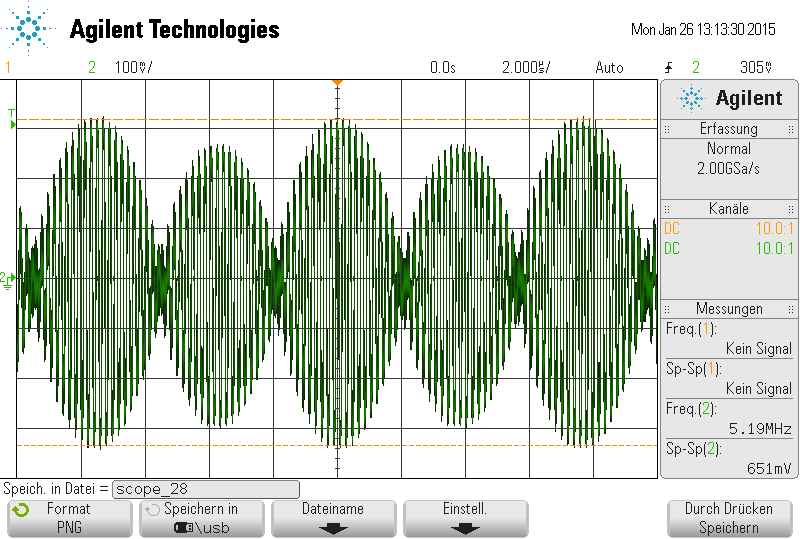
\includegraphics[width=0.9\linewidth]{images/am-signal.png}
    \caption{Amplitudenmoduliertes Signal.}
    \label{fig:am-signal}
\end{figure}
\begin{figure}
    \centering
    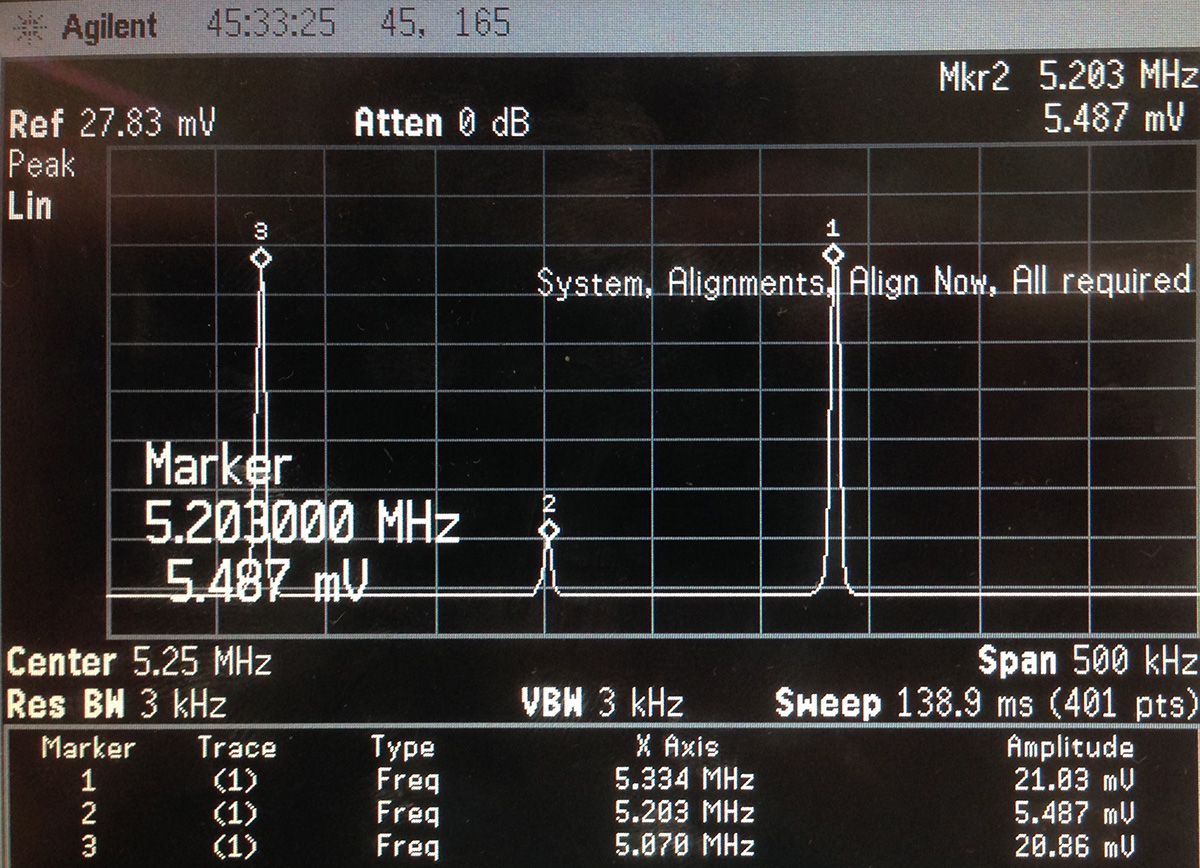
\includegraphics[width=0.9\linewidth]{images/am-spektrum.jpg}
    \caption{
        Frequenzspektrum des AM-Signals im Bereich um die
        Trägerfrequenz.
    }
    \label{fig:am-spektrum}
\end{figure}

\subsubsection{Amplitudenmodulation mit Diode}
\label{subsubsec:am-ringmodulator}
Die Amplitudenmodulation mit Hilfe einer Diode liefert das in Abbildung
\ref{fig:am-diode-signal}, beziehungsweise \ref{fig:am-diode-spektrum}
dargestellte Signal und Spektrum. Die Oberwellen der Trägerfrequenz bei
$2\omega_\text{T} = \SI{10}{\mega\hertz}$ und
$3\omega_\text{T} = \SI{15}{\mega\hertz}$ treten auf, weil XXX.
Sie sind in Abbildung \ref{fig:am-diode-oberwellen}

Der Modulationsgrad $m$ beträgt nach Gleichung XXX
\begin{equation*}
    m = \num{1}\,.
\end{equation*}
\begin{figure}
    \centering
    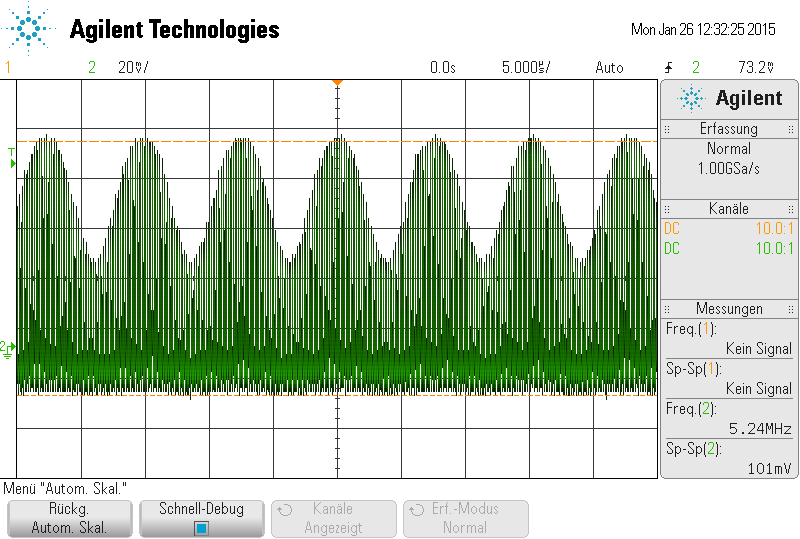
\includegraphics[width=0.9\linewidth]{images/am-diode-signal.png}
    \caption{Mit Hilfe einer Diode moduliertes Signal.}
    \label{fig:am-diode-signal}
\end{figure}
\begin{figure}
    \centering
    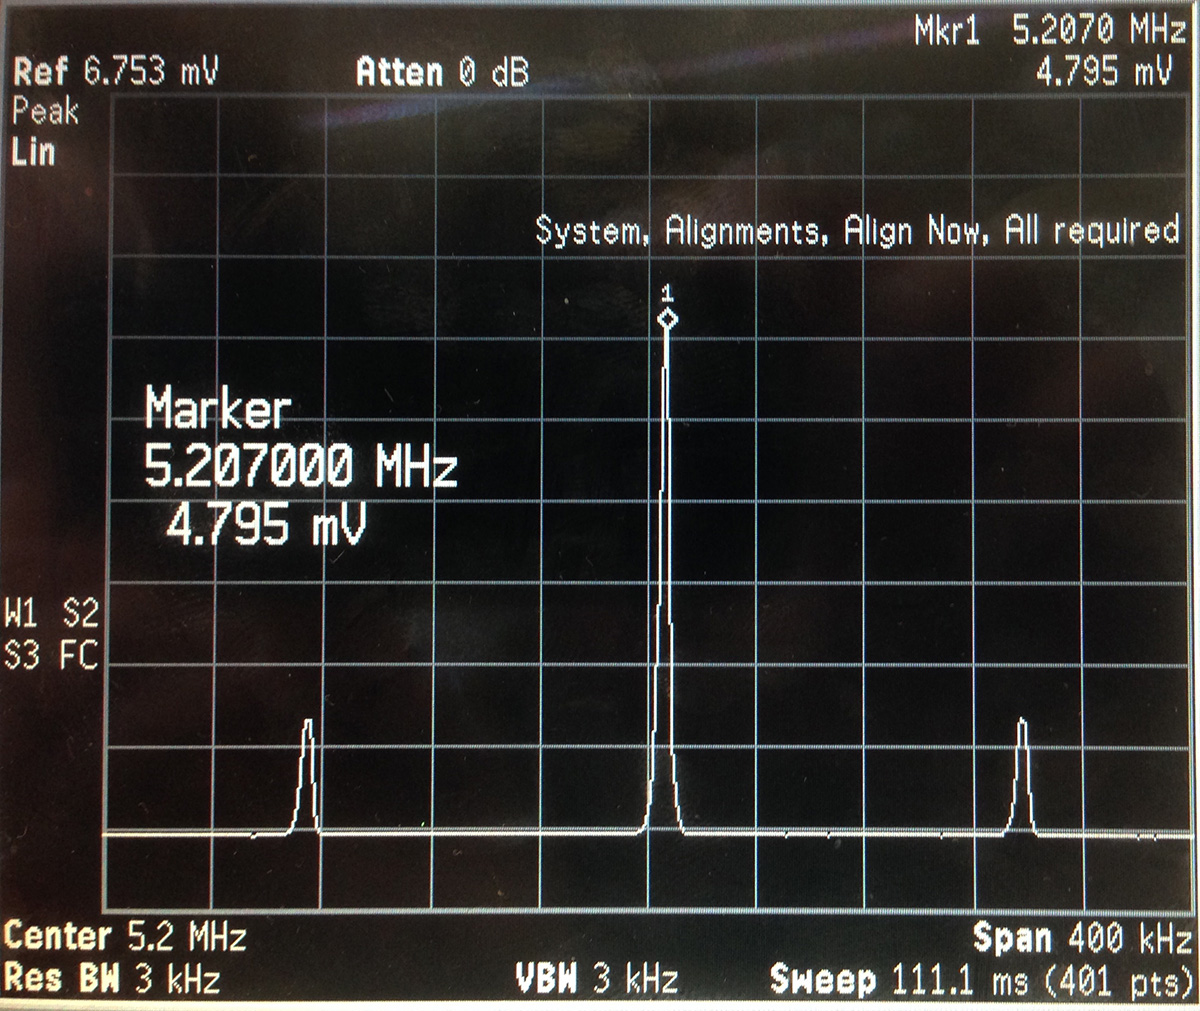
\includegraphics[width=0.9\linewidth]{images/am-diode-spektrum.jpg}
    \caption{
        Frequenzspektrum des mit Hilfe einer Diode erzeugten AM-Signals im
        Bereich um die Trägerfrequenz.
    }
    \label{fig:am-diode-spektrum}
\end{figure}
\begin{figure}
    \centering
    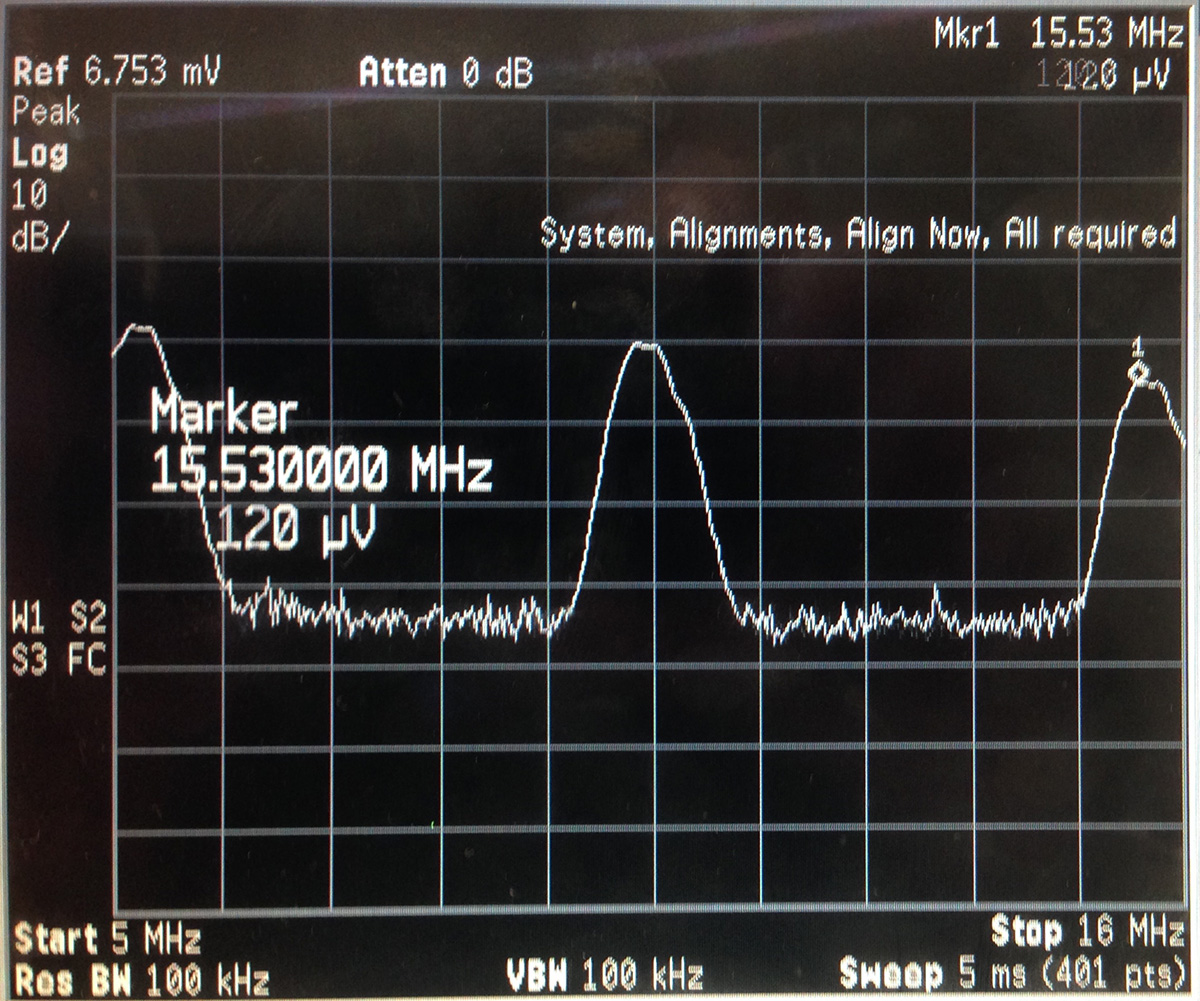
\includegraphics[width=0.9\linewidth]{images/am-diode-oberwellen.jpg}
    \caption{
        Oberwellen des AM-Singals.
    }
    \label{fig:am-diode-oberwellen}
\end{figure}
